\documentclass[11pt, oneside]{article}
\usepackage{geometry}
\usepackage{verbatim}
\geometry{letterpaper}
%\geometry{landscape}                   % Activate for for rotated page geometry
\usepackage[parfill]{parskip}
\usepackage{graphicx} 
\usepackage{hyperref} 
\usepackage{amssymb}
\usepackage{amstext}
\usepackage{color}
\usepackage{float}
\newcommand{\hilight}[1]{\colorbox{yellow}{#1}}
\newcommand{\question}[3]{ 
  \section{#1:} 
  \subsection*{Question:} #2
  \subsection*{Solution:} #3 
} 
\title{CS5800: Assignment 3}
\author{Patrick Loftus}
\date{01/28/2015}
\begin{document}
\begin{titlepage}
\maketitle
\tableofcontents
\thispagestyle{empty}
\end{titlepage}

%%%%%%%%%%%%%%%%%%%%%% Chapter 2 %%%%%%%%%%%%%%%%%%%%%%
\question{5.1}
{
  Give a clear English description of the language accepted by the DFSM on page
  121 of Rich.
}
{
  The DFSM requires the input string to meet 2 requirements:
  \begin{enumerate}
    \item contains at least 1 b
    \item contains either 0 a's or a substring of an odd number of repeated a's
  \end{enumerate}
}

\question{5.2}
{
  Show a DFSM to accept each of the following languages:
  \begin{enumerate}
    \item[a.]
      $L = \left\{ w \in \left\{ a,b \right\}^*: 
      \text{
        every $a$ in $w$ is immediately preceded and followed by b.
      }\right\}$.
    \item[b.]
      $L = \left\{ w \in \left\{ a,b \right\}^*: 
      \text{
        $w$ does not end in $ba$
      }\right\}$.
    \item[c.]
      $L = \left\{ w \in \left\{ 0,1 \right\}^*: 
      \text{
        $w$ corresponds to the binary encoding without leading $0$'s of natural
        numbers that are evenly divisible by $4$.
      }\right\}$.
    \item[d.]
      $L = \left\{ w \in \left\{ 0,1 \right\}^*: 
      \text{
        $w$ corresponds to the binary encoding without leading $0$'s of natural
        numbers that are powers of $4$.
      }\right\}$.
    \item[e.]
      $L = \left\{ w \in \left\{ 0-9 \right\}^*: 
      \text{
        $w$ corresponds to the binary encoding without leading $0$'s of an odd
        natural number
      }\right\}$.
    \item[f.]
      $L = \left\{ w \in \left\{ 0,1 \right\}^*: 
      \text{
        $w$ has $001$ as a substring.
      }\right\}$.
    \item[g.]
      $L = \left\{ w \in \left\{ 0,1 \right\}^*: 
      \text{
        $w$ does not have $001$ as a substring.
      }\right\}$.
    \item[h.]
      $L = \left\{ w \in \left\{ a,b \right\}^*: 
      \text{
        $w$ has $bbab$ as a substring
      }\right\}$.
    \item[i.]
      $L = \left\{ w \in \left\{ a,b \right\}^*: 
      \text{
        $w$ has neither $bb$ nor $ab$ as a substring
      }\right\}$.
    \item[j.]
      $L = \left\{ w \in \left\{ a,b \right\}^*: 
      \text{
        $w$ has both $bb$ and $ab$ as a substring
      }\right\}$.
    \item[k.]
      $L = \left\{ w \in \left\{ a,b \right\}^*: 
      \text{
        $w$ contains at least 2 $b$'s that are not immediately followed by an
        $a$
      }\right\}$.
    \item[l.]
      $L = \left\{ w \in \left\{ 0,1 \right\}^*: 
      \text{
        $w$ has no more than one pair of consecutive $0$'s and no more than one
        pair of consecutive $1$'s.
      }\right\}$.
    \item[m.]
      $L = \left\{ w \in \left\{ 0,1 \right\}^*: 
      \text{
        $w$ none of the prefixes of $w$ ends in $0$
      }\right\}$.
    \item[n.]
      $L = \left\{ w \in \left\{ 0,1 \right\}^*: 
        (\#_a(w) + 2 \cdot \#_b(w)) \equiv_5 0
      \right\}$.
  \end{enumerate}
} 
{
  \begin{enumerate}
    \item[a.] 
      \begin{minipage}{\linewidth}
        \centering
        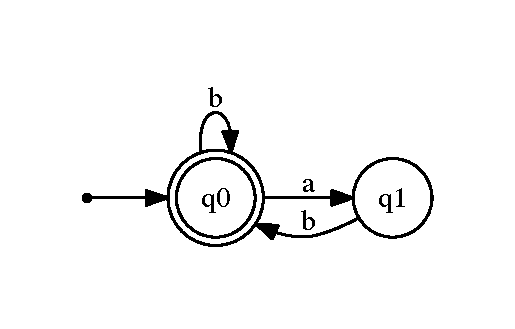
\includegraphics[width=0.8\textwidth,natwidth=610,natheight=642]{5_2_a.pdf}
      \end{minipage}
    \item[b.] 
      \begin{minipage}{\linewidth}
        \centering
        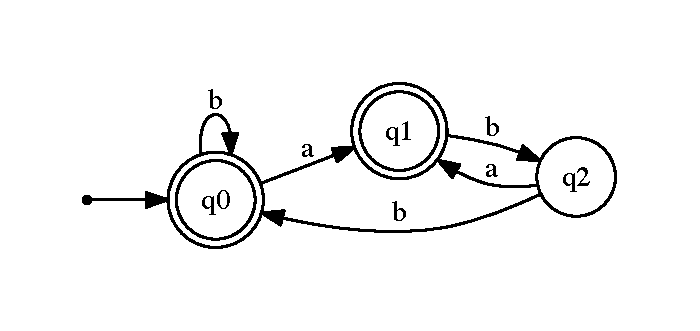
\includegraphics[width=0.8\textwidth,natwidth=610,natheight=642]{5_2_b.pdf}
      \end{minipage}
    \item[c.]
      \begin{minipage}{\linewidth}
        \centering
        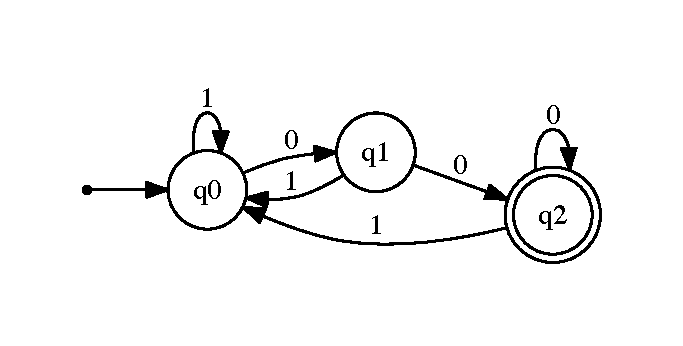
\includegraphics[width=0.8\textwidth,natwidth=610,natheight=642]{5_2_c.pdf}
      \end{minipage}
    \item[d.]
      \begin{minipage}{\linewidth}
        \centering
        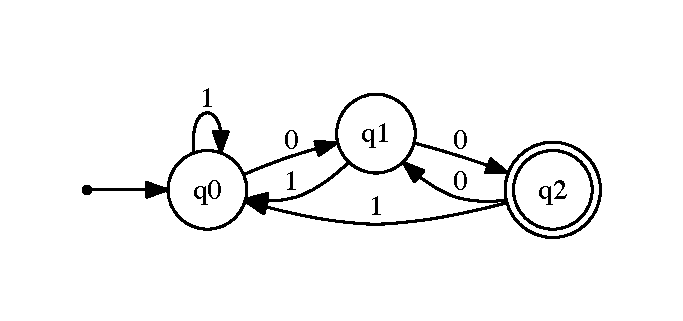
\includegraphics[width=0.8\textwidth,natwidth=610,natheight=642]{5_2_d.pdf}
      \end{minipage}
    \item[e.]
      \begin{minipage}{\linewidth}
        \centering
        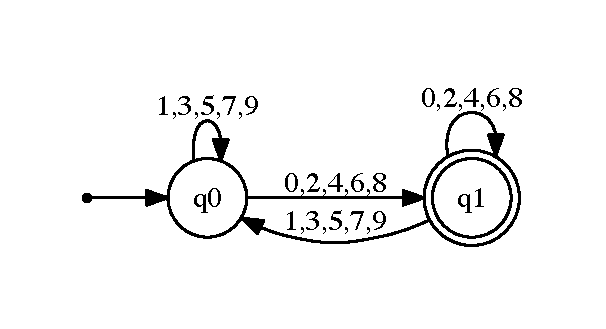
\includegraphics[width=0.8\textwidth,natwidth=610,natheight=642]{5_2_e.pdf}
      \end{minipage}
    \item[f.]
      \begin{minipage}{\linewidth}
        \centering
        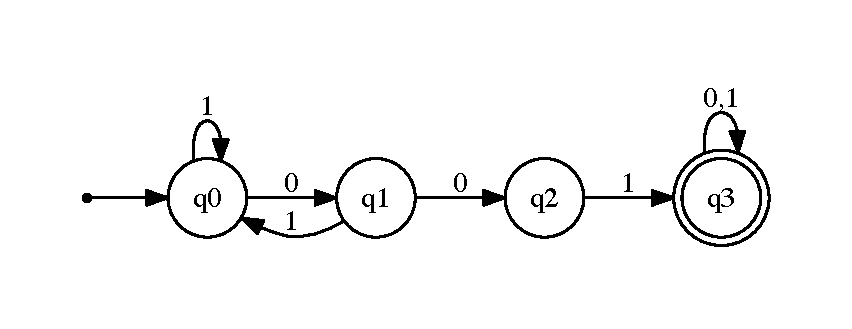
\includegraphics[width=0.8\textwidth,natwidth=610,natheight=642]{5_2_f.pdf}
      \end{minipage}
    \item[g.]
      \begin{minipage}{\linewidth}
        \centering
        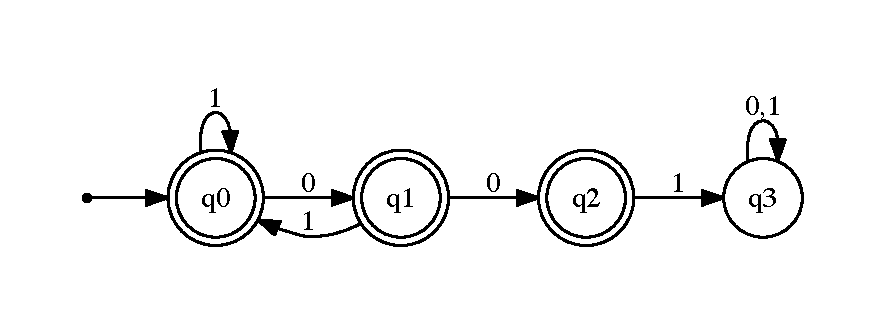
\includegraphics[width=0.8\textwidth,natwidth=610,natheight=642]{5_2_g.pdf}
      \end{minipage}
    \item[h.]
      \begin{minipage}{\linewidth}
        \centering
        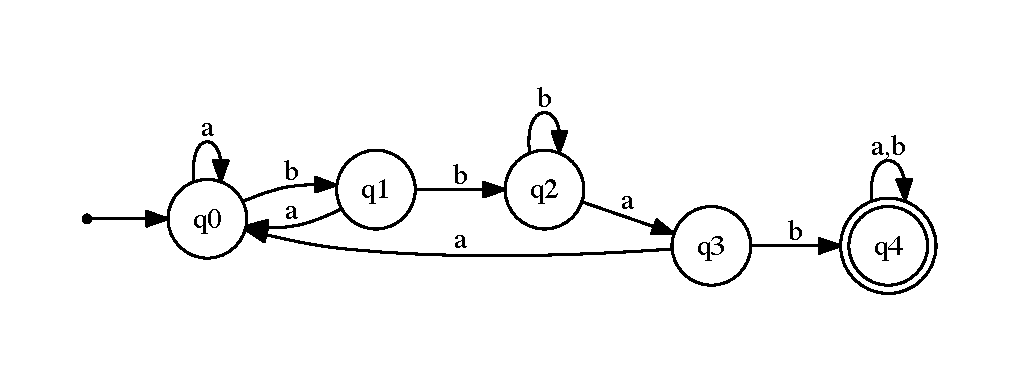
\includegraphics[width=0.8\textwidth,natwidth=610,natheight=642]{5_2_h.pdf}
      \end{minipage}
    \item[i.]
      \begin{minipage}{\linewidth}
        \centering
        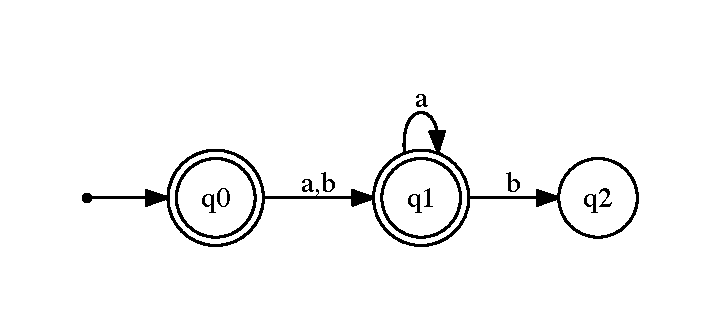
\includegraphics[width=0.8\textwidth,natwidth=610,natheight=642]{5_2_i.pdf}
      \end{minipage}
    \item[j.]
      \begin{minipage}{\linewidth}
        \centering
        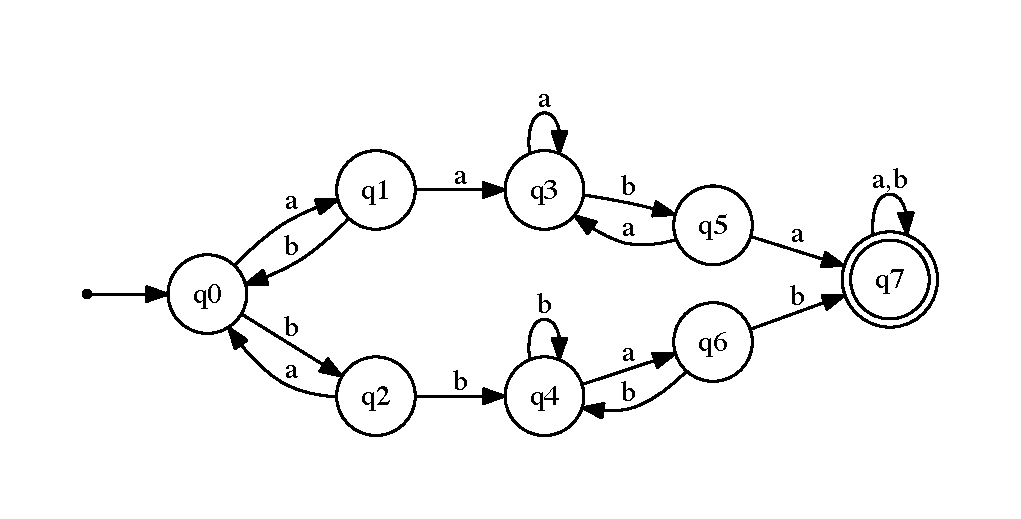
\includegraphics[width=0.8\textwidth,natwidth=610,natheight=642]{5_2_j.pdf}
      \end{minipage}
    \item[k.]
      \begin{minipage}{\linewidth}
        \centering
        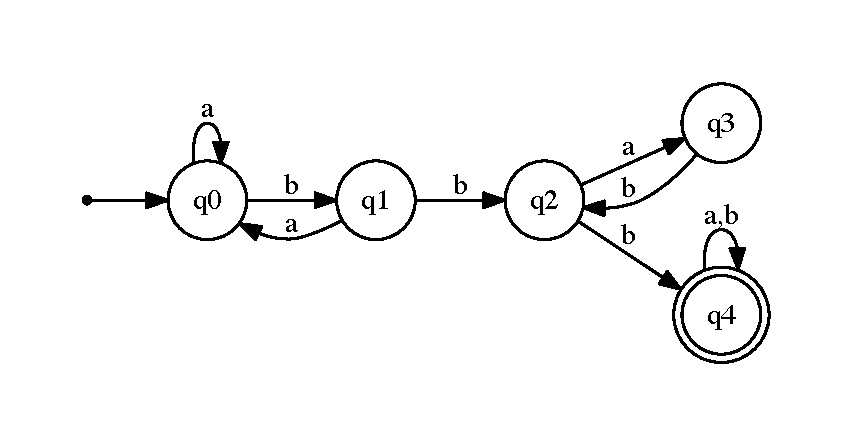
\includegraphics[width=0.8\textwidth,natwidth=610,natheight=642]{5_2_k.pdf}
      \end{minipage}
    \item[l.]
      \begin{minipage}{\linewidth}
        \centering
        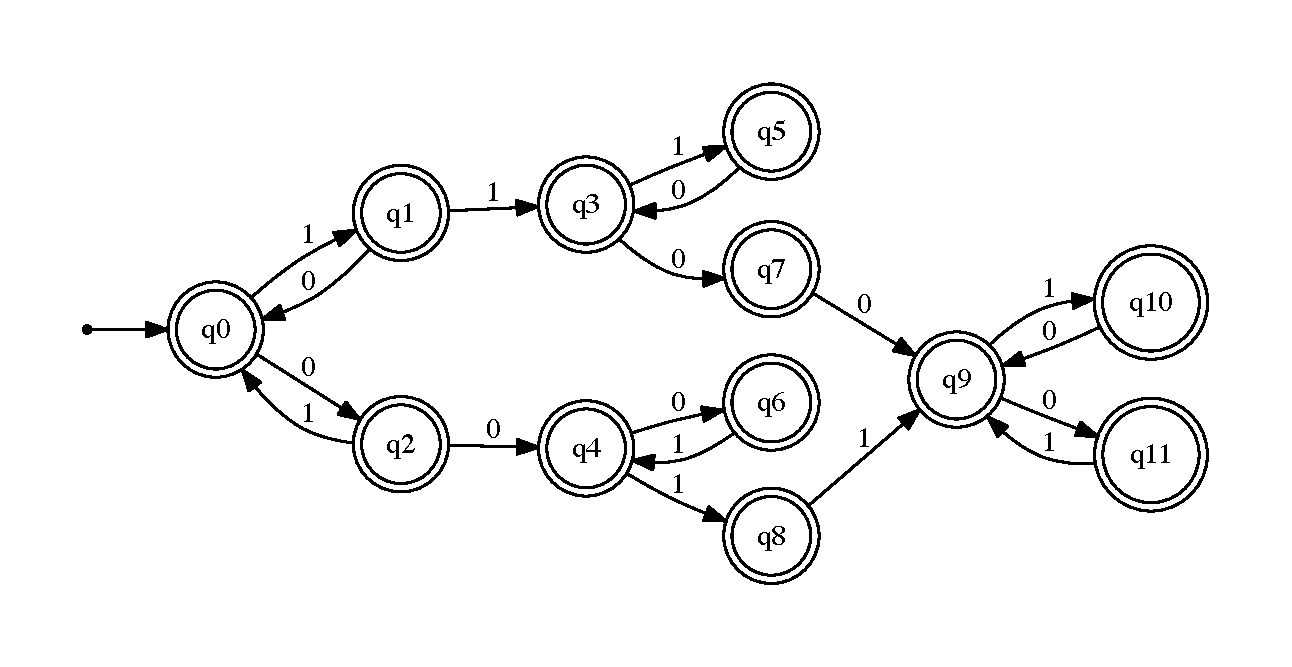
\includegraphics[width=0.8\textwidth,natwidth=610,natheight=642]{5_2_l.pdf}
      \end{minipage}
    \item[m.]
      \begin{minipage}{\linewidth}
        \centering
        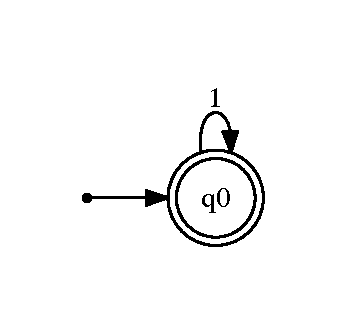
\includegraphics[width=0.8\textwidth,natwidth=610,natheight=642]{5_2_m.pdf}
      \end{minipage}
    \item[n.]
      \begin{minipage}{\linewidth}
        \centering
        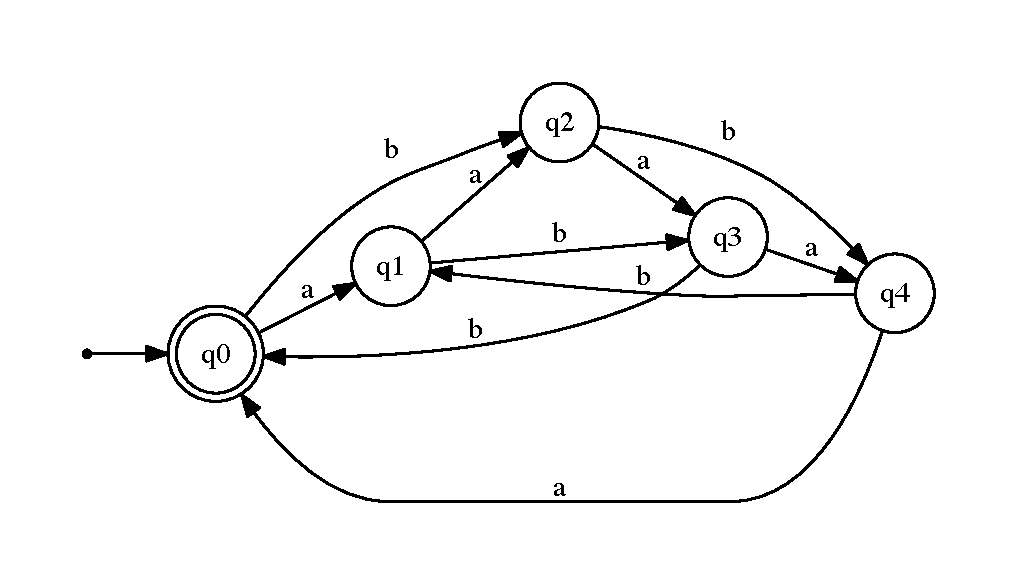
\includegraphics[width=0.8\textwidth,natwidth=610,natheight=642]{5_2_n.pdf}
      \end{minipage}
  \end{enumerate}
}

\question{5.3}
{
  Consider the children's game Rock, Paper, Scissors.  We'll say that the first
  player to win two rounds wins the game.  Call the two players $A$ and $B$.
  \begin{enumerate}
    \item[a.]
      Define an alphabet $\Sigma$ and describe a technique for encoding rock,
      paper, scissors games as strings over $\Sigma$.
    \item[b.]
      Let $L_{RPS}$ be the language described in part $a$ that correspond to wins
      for player $A$.  Show a DFSM that accepts $L_{RPS}$
  \end{enumerate}
}
{
  \begin{enumerate}
    \item[a.]
      Let:\\
      \begin{tabular}{c | c | c}
        encoding & $A$ & $B$\\
        \hline
        0 & rock     & rock     \\
        1 & rock     & paper    \\
        2 & rock     & scissors \\
        3 & paper    & rock     \\
        4 & paper    & paper    \\
        5 & paper    & scissors \\
        6 & scissors & rock     \\
        7 & scissors & paper    \\
        8 & scissors & scissors \\
      \end{tabular}
      \\Using this encoding, we can describe any number of rock, paper, scissors games 
      as strings in the language 
      $L_{RPS} = \left\{ w \in \left\{ 0-8 \right\}^*    \right\}$.
    \item[b.]
      \begin{minipage}{\linewidth}
        \centering
        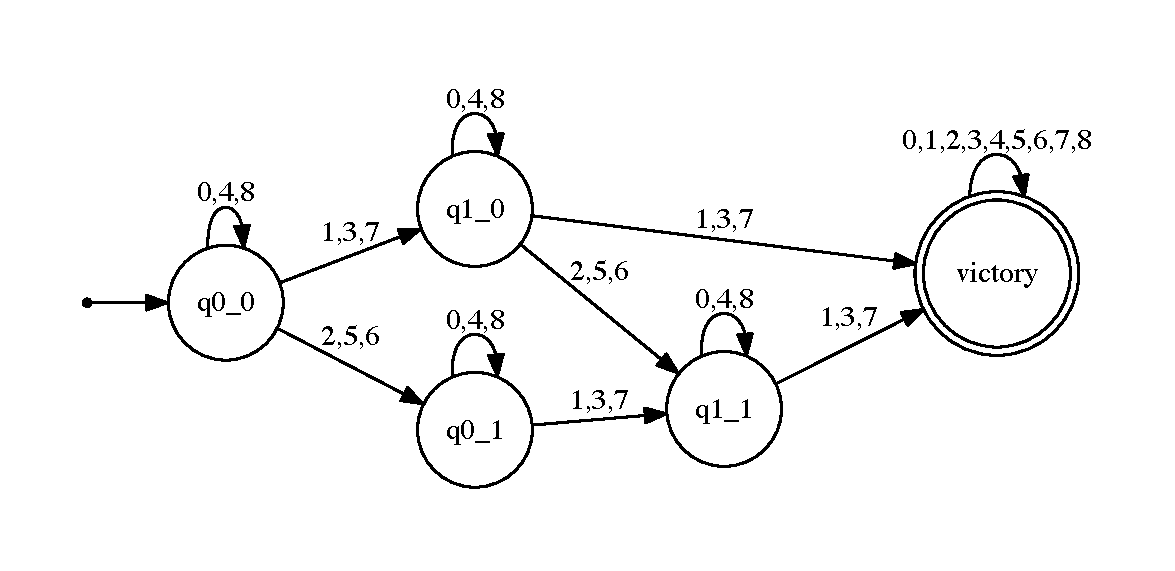
\includegraphics[width=0.8\textwidth,natwidth=610,natheight=642]{5_3_b.pdf}
      \end{minipage}
  \end{enumerate}
}

\question{5.4}
{
  If $M$ is a DFSM and $\varepsilon \in L(M)$, what simple property must be ture
  of $M$?
}
{
  The start state must be an accepting state.
}

\end{document}
